


\documentclass[runningheads,a4paper]{llncs}

\usepackage{amssymb}
\setcounter{tocdepth}{3}
\usepackage{graphicx}
\usepackage{url}

%Preamble File for Random Regression Paper

%\usepackage{times}

%Theorems and such

%\usepackage{amsthm}

%\newtheorem{theorem}{Theorem}
%\newtheorem{observation}{Observation}
%\newtheorem{proposition}{Proposition}
%\newtheorem{definition}{Definition}

%\newtheorem{theorem}{Theorem}[section]
%\newtheorem{observation}{Observation}[section]
%\newtheorem{proposition}{Proposition}[section]
%\newtheorem{definition}{Definition}[section]

\usepackage[ruled,vlined]{algorithm2e}
\usepackage{algorithmic}
%\usepackage{amsthm}
\usepackage{amsmath}
\usepackage{amsfonts}
\usepackage{amssymb}
\usepackage{graphicx}
\usepackage{url}
\usepackage{subfigure}
\usepackage{epstopdf}
%\setcounter{MaxMatrixCols}{30}
%\usepackage[ruled,vlined]{algorithm2e}
%\usepackage{algorithmic}
\usepackage{multirow}
\usepackage{subfigure}
\usepackage{ifthen}
\DeclareMathOperator*{\argmax}{argmax}
\DeclareMathOperator*{\argmin}{argmin}
%\DeclareMathOperator{\pattern}{\pi}
\DeclareMathOperator{\Poly}{\mathbf{\mathrm{P}}}
\DeclareMathOperator{\RP}{\mathbf{\mathrm{RP}}}
%\DeclareMathOperator{\FP}{\mathbf{\mathrm{FP}}}
\DeclareMathOperator{\NP}{\mathbf{\mathrm{NP}}}
%\DeclareMathOperator{\E}{\mathbb{E}}

\newcommand{\defterm}{\textbf}

\renewcommand{\d}{\mathbf{d}}

\newcommand{\ZZ}{\mathbf{Z}}

\newcommand{\indep}{\ensuremath{\perp{}\!\!\!\!\!\!\!\perp{}}}
\newcommand{\dep}{\ensuremath{{\perp{}\!\!\!\!\!\!\!\not  \perp{}}}}
%\renewcommand{\L}{\mathcal{L}}

% variables denoting sets of nodes
\newcommand{\BN}{B} % Bayes net
\newcommand{\V}{V} 
\newcommand{\partC}{\mathcal{C}}
\newcommand{\pattern}{\pi}
% for population variables
\newcommand{\A}{\mathbb{A}}
\newcommand{\B}{\mathbb{B}}
\newcommand{\C}{\mathbb{C}}
\newcommand{\U}{\mathbb{U}}
%maybe use P, R as well??
\renewcommand{\P}{P}
\newcommand{\R}{R}
% values of Pop variables = constants
\renewcommand{\a}{a}
\renewcommand{\b}{b}
\renewcommand{\c}{c}

%%%
% for terms = nodes in Functor Bayes Net.
\newcommand{\X}{X}
\newcommand{\Y}{Y}
\newcommand{\Z}{Z}
% Next three are currently only ones eligible for \Mrange and \Prange
\newcommand{\TT}{T}
\newcommand{\TI}{\mathsf{T}}
\newcommand{\UT}{U}
\newcommand{\UI}{\mathsf{U}}
\newcommand{\VT}{V}
\newcommand{\VI}{\mathsf{V}}
\newcommand{\W}{W}
%syntax for values
\newcommand{\z}{z}
\renewcommand{\v}{v}
\newcommand{\x}{x}
\newcommand{\y}{y}
\newcommand{\p}{p}
\newcommand{\s}{s}
% Values tied to terms
\newcommand{\TV}{t}
\newcommand{\TTuple}[1][0.0ex]{\vec{t}\hspace{#1}}
\newcommand{\UV}{u}
\newcommand{\UTuple}[1][0.0ex]{\vec{u}\hspace{#1}}
\newcommand{\VV}{v}
\newcommand{\VTuple}{\vec{v}}
%%%
\newcommand{\weight}{w} % weights
% Formulas
\newcommand{\TF}{\vec{T}}
\newcommand{\UF}{\vec{U}}
\newcommand{\VF}{\vec{V}}
%\newcommand{\TF}{\phi}
%\newcommand{\UF}{\psi}
%\newcommand{\VF}{\omega}
% Database (which is always fully-grounded)
\newcommand{\DB}{\FG{\Delta}}
\newcommand{\QC}{\FG{\Lambda}}
\newcommand{\QCtarget}{\FG{\Lambda_{-\TI}}}
% to define a query conjunction of literals
\newcommand{\Qconj}{\Appendterm{\FG{\TT_{\grounding}} = \TV} {\QC}}

% Annotations marking degree of grounding
\newcommand{\UG}[2][0.0ex]{#2^{-}\hspace{#1}}
\newcommand{\PG}[2][0.0ex]{#2^{\prime}\hspace{#1}}
\newcommand{\FG}[2][0.0ex]{#2^{*}\hspace{#1}}

% Functions returning related terms
\newcommand{\MB}[1]{\mathrm{MB}(#1)}
\newcommand{\Pa}[1]{\mathrm{Pa}(#1)}
\newcommand{\Ch}[1]{\mathrm{Ch}(#1)}

% Grounding
\newcommand{\Ground}[1]{#1_\gamma}
\newcommand{\gndlink}{\backslash}

% Values in ranges of example functors
\newcommand{\Man}{\mathrm{M}}
\newcommand{\Woman}{\mathrm{W}}

% Adding a term to a formula
\newcommand{\sepcup}[1][0.5ex]{\hspace{#1}\cup\hspace{#1}}
\newcommand{\Setaddterm}[2]{#1 \sepcup #2}
\newcommand{\Appendterm}[2]{#1, #2}

% Values in the range of related terms
\newcommand{\Mrange}[1]{\ifthenelse{\equal{#1}{T}}{\TTuple_m}{\ifthenelse{\equal{#1}{U}}{\UTuple_m}{\ifthenelse{\equal{#1}{V}}{\VTuple_m}{\mbox{UNKNOWN
TERM ID}}}}}
\newcommand{\Prange}[1]{\ifthenelse{\equal{#1}{T}}{\vec{t}_{pa}}{\ifthenelse{\equal{#1}{U}}{\vec{u}_{pa}}{\ifthenelse{\equal{#1}{V}}{\vec{v}_{pa}}{\mbox{UNKNOWN
TERM ID}}}}}

\newcommand{\GroundPrange}[1]{\ifthenelse{\equal{#1}{T}}{\vec{t}_{pa,\grounding'}}{\ifthenelse{\equal{#1}{U}}{\vec{u}_{pa,\grounding'}}{\ifthenelse{\equal{#1}{V}}{\vec{v}_{pa,\grounding'}}{\mbox{UNKNOWN
TERM ID}}}}}


% Key functions
\newcommand{\joint}{p}
\newcommand{\jprob}[1]{\theta(#1)}
\newcommand{\cprob}[2]{\theta(#1|#2)}
\newcommand{\estcprob}[3]{\widehat{\theta}(#1|#2;#3)}
%\newcommand{\Gpvar}{\tilde{P}}
\newcommand{\Gpvar}{P}
\newcommand{\Gprob}[2]{\Gpvar(#1 | #2)}
\newcommand{\QFC}{QFC} % query family configuration
\newcommand{\Cvar}{\mathrm{n}}
\newcommand{\Fvar}{\mathrm{p}}
\newcommand{\Count}[2]{\Cvar\left[#1;#2\right]}
\newcommand{\CountC}[3]{\Cvar_{#3}\left[#1;#2\right]}
\newcommand{\Freq}[2]{\Fvar\left[#1;#2\right]}
\newcommand{\Relevant}[1]{#1^{\mathrm{r}}}
\newcommand{\Relcount}[2]{\Relevant{\Cvar}\left[#1;#2\right]}
\newcommand{\RelcountC}[3]{\Relevant{\Cvar_{#3}}\left[#1;#2\right]}
\newcommand{\Relfreq}[2]{\Relevant{\Fvar}\left[#1;#2\right]}
\newcommand{\RelfreqC}[3]{\Relevant{\Fvar_{#3}}\left[#1;#2\right]}
\newcommand{\Range}[1]{\mathrm{Ra}(#1)}
\newcommand{\Vars}[1]{\mathrm{Va}(#1)}
% no longer needed
%\newcommand{\Crossprod}[1]{\mathcal{X}}

%variables for sets of values
\newcommand{\setx}{\set{x}}
\newcommand{\sety}{\set{y}}
\newcommand{\setz}{\set{z}}


%statistics
\newcommand{\score}{S}
\newcommand{\parameters}{\mathit{par}}
\newcommand{\bic}{\mathit{BIC}}
%random variables and graphical models
% number of values in the domain of a random variable
% variables for BNs
\newcommand{\domvals}{k}
\newcommand{\nodevalue}{\x}
\newcommand{\parvalue}{\mathbf{\pi}} % a single assignment of values to a set of 
%parents
\newcommand{\parvals}{l} % number of values of parent state.
\renewcommand{\r}{r} % CP-table row
\newcommand{\nbhd}{{\mathsf {nbdh}}}
\newcommand{\child}{\mathit{child}}
\newcommand{\parent}{\mathit{pa}}
\newcommand{\parents}{\mathbf{pa}}
\newcommand{\Parents}{\mathbf{PA}}
\newcommand{\family}{F} % families, family formulas
\newcommand{\Target}{Y_{\target}}
\newcommand{\MBtarget}{\set{X}_{\target}} % Markov blanket of a target node.
\newcommand{\mbtarget}{\set{x}} % values for the markov blanket of a variable, vector-valued
\newcommand{\mbstates}{m} % number of states in Markov blanket
\newcommand{\vpi}{\mathbf{pa}} % for vectors of variable assignments
\renewcommand{\l}{\ell} % class label
\newcommand{\states}{r} % number of states of a variable
\newcommand{\ssize}{N} % number of rows in join table; size of sample
\newcommand{\frequency}{fr}
\newcommand{\pseudo}{\ast}
\newcommand{\counts}{+}
\newcommand{\weighted}{\ast}
\newcommand{\halpern}{H}
\newcommand{\instance}{I}

%logic notation
\newcommand{\functor}{f}
\newcommand{\fvalue}{v}
\newcommand{\variable}{X} % first-order variable
\newcommand{\population}{\mathcal{P}}
\newcommand{\entity}{x}
\newcommand{\formula}{\phi}
\newcommand{\formulas}{\mathcal{\phi}}
\newcommand{\conjunction}{\set{C}} % 
\newcommand{\outdomain}{V}
\newcommand{\literal}{\ell}
%conjunction of literals
\newcommand{\fterm}{\f} % open function term
\newcommand{\fterms}{F} % set of function terms, also nodes in JBN
\newcommand{\term}{\tau}
\newcommand{\terms}{\bs{\tau}}
\newcommand{\constant}{a}
\newcommand{\constants}{\bs{\constant}}
\newcommand{\gterm}{g} % ground term
\newcommand{\gterms}{\bs{\gterm}} %list of ground terms
\newcommand{\vterm}{x} % variable term
\newcommand{\vterms}{\bs{\vterm}} % list of variable terms
\newcommand{\assign}{A} % assignment of values to Bayes net
\newcommand{\grounds}{\#}
\newcommand{\grounding}{\gamma}
\newcommand{\groundall}{\Gamma}
\newcommand{\vars}{\mathit{Var}} % variables in a conjunction
\newcommand{\igraph}{I} % instance-level dependency graph.
\newcommand{\assignment}{\set{a}}
\newcommand{\atom}{\functor}
\newcommand{\gnode}{\alpha}
\newcommand{\gfamily}{\ground{f}}
\newcommand{\numformulas}{m}
% logic programs
\newcommand{\program}{\mathcal{B}}
\newcommand{\clause}{\mathcal{c}}
\newcommand{\head}{\mathit{head}}
\newcommand{\body}{\mathit{body}}
\newcommand{\crule}{\mathit{cr}} % combining rule
\newcommand{\level}{\mathit{level}} % rank of function symbols in LP

%datbase schema
\newcommand{\rcolumns}{R}
\newcommand{\ecolumns}{E}
\newcommand{\dtable}{T} % can't use \table. Generic database table
\newcommand{\datatable}{D} % generic data table, not necessarily part of database.
\newcommand{\jtable}{J} % join table
\newcommand{\Ejoin}{$J^{+}$}
\newcommand{\jtables}{m}
\newcommand{\rtable}{R} % relationship table
\newcommand{\etable}{E} % entity table.
\newcommand{\ttable}{X} % target table
\newcommand{\nextended}{n}
\newcommand{\row}{r}
\newcommand{\rows}{\mathit{rows}}
\newcommand{\col}{j}
\newcommand{\cols}{\mathit{cols}}
\newcommand{\unary}{\f} % to denote a unary or attribute function
\newcommand{\numatts}{u} % to denote the number of unary or attribute functions.
\newcommand{\g}{g} % alternative for function
\newcommand{\relational}{\mathbf{r}} % denotes a generic relational functors, can be both relationship or descriptive attribute of relationship
\newcommand{\Relation}{R} % denotes a generic boolean relation
% a special type of literal conjunction that assigns a value %to each variable
\newcommand{\class}{c} % the class attribute
\newcommand{\classifier}{\mathcal{C}}
\newcommand{\target}{t} % target object
\newcommand{\feature}{f} % feature or desc attribute of object or link
\newcommand{\features}{\bs{f}} % features 
\newcommand{\attribute}{a} % nonclass attribute of target object
\newcommand{\attributes}{\bs{a}}
\newcommand{\rels}{\bs{R}} % chain of relationships.
\newcommand{\maxpath}{\rho}

%special functions
\newcommand{\AVG}{\it{AVG}}
\newcommand{\instances}{n} % counts number of occurrences in DB
\newcommand{\prob}{p} % frequency of formula true in in DB

%variables denoting graphs or models
\newcommand{\mln}{M}
\newcommand{\G}{G}
\newcommand{\node}{X}
\newcommand{\nodes}{V}
\newcommand{\edges}{E}
\newcommand{\clique}{C}
\newcommand{\cliques}{\mathcal{\clique}}
\newcommand{\cliquevalue}{c}
\newcommand{\graph}{G}
\newcommand{\M}{M}
\newcommand{\J}{J}
\renewcommand{\H}{H}
\newcommand{\K}{K} % component
\renewcommand{\O}{O} % oracle
\renewcommand{\path}{\rho} % path, also foreignkey path
% Markov nets
\newcommand{\potential}{\Psi}
% database schema
\newcommand{\type}{\tau} % to denote a generic type
\newcommand{\E}{E} % for entity tables
\newcommand{\e}{e} % for specific entities
\newcommand{\f}{f}
\newcommand{\new}{\it{new}}
\renewcommand{\c}{c}
\renewcommand{\R}{R} % for relationship tables
%\newcommand{\A}{A} % for attributes
\newcommand{\T}{T} % for tables generically
\newcommand{\New}{N}
\newcommand{\D}{\mathcal{D}} % for database instance
\renewcommand{\S}{\mathcal{S}} % for relational structure as conjunction of literals
\newcommand{\databases}{\set{D}} % the number of databases
\newcommand{\vocab}{\mathcal{\L}} % for logical vocabulary associated with database
\newcommand{\name}{\mathit{name}} % generic attribute
\newcommand{\dom}{\mathit{dom}} % domain of attributes
\newcommand{\etables}{\alpha} % entity tables
\newcommand{\rtables}{\beta} % relationship table number
% specific constructs for examples
\newcommand{\student}{\mathit{Student}}
\newcommand{\I}{\mathit{I}}
\newcommand{\course}{C}
\newcommand{\prof}{\mathit{Professor}}
\newcommand{\person}{\mathit{Person}}
\newcommand{\TA}{\mathit{TA}}
\newcommand{\actor}{\mathit{Actor}}
\newcommand{\age}{\mathit{age}}
\newcommand{\intelligence}{\mathit{intelligence}}
\newcommand{\diff}{\mathit{difficulty}}
\newcommand{\reg}{\mathit{Registered}}
\newcommand{\ra}{\mathit{RA}}
\newcommand{\bt}{\mathit{blood type}}
\newcommand{\grade}{\mathit{grade}}
\newcommand{\gpa}{\mathit{gpa}}
\newcommand{\jack}{\mathit{Jack}}
\newcommand{\jill}{\mathit{Jill}}
\newcommand{\smith}{\mathit{Smith}}
\newcommand{\cmpt}{\mathit{CMPT120}}
\newcommand{\hi}{\mathit{Hi}}
% various constants
\newcommand{\true}{\mathrm{T}}
\newcommand{\false}{\mathrm{F}}
\newcommand{\normalconstant}{Z} % the normalization constant

% orderings
\newcommand{\pred}{\mathit{pred}}
%procedure names and such
\newcommand{\join}{\textsc{Join-Frequencies}}
\newcommand{\linus}{\textsc{Linus }}
\newcommand{\foil}{\textsc{Foil }}
\newcommand{\MLN}{\textsc{MLN}}
\newcommand{\treetilde}{\textsc{TILDE }}

%%%
%undirected models
\newcommand{\pot}{\phi} % potential function
%\newcommand{\theHalgorithm}{\arabic{algorithm}}
\newcommand{\test}{test}
\def\set#1{\mathbf{#1}}
\def\bs#1{\boldsymbol{#1}}
\def\ground#1{\overline{#1}}


\begin{document}

\mainmatter  % start of an individual contribution

% first the title is needed
\title{Learning Bayes Nets for Relational Data With Link Uncertainty}
% a short form should be given in case it is too long for the running head
\titlerunning{Relational Bayes Nets With Link Uncertainty}


\author{Zhensong Qian and Oliver Schulte
\thanks{
This research was supported by a Discovery Grant to Oliver Schulte from the Canadian Natural Sciences and Engineering Council. 
And Zhensong Qian was also supported by a grant from the China Scholarship Council.
The preliminary version of this paper was presented in the IJCAI 2013 GKR workshop.
}
 }

\institute{ School of Computing Science\\ Simon Fraser University\\Vancouver-Burnaby, Canada\\
\{zqian,oschulte\}@sfu.ca\\
\url{http://www.cs.sfu.ca/~oschulte/}}


\maketitle


\begin{abstract} 
We present an algorithm for learning correlations among link types and node attributes in relational data that represent complex networks. 
The link correlations are represented in a Bayes net structure. This provides a succinct graphical way to display relational statistical patterns and support powerful probabilistic inferences. The current state of the art algorithm for learning relational Bayes nets captures only correlations among entity attributes {\em given} the existence of links among entities. The models described in this paper capture a wider class of correlations that involve uncertainty about the link structure. Our base line method learns a Bayes net from join tables directly. This is  a statistically powerful procedure that finds many correlations, but does not scale well to larger datasets. We compare join table search with a hierarchical search strategy.
\end{abstract}


\section{Introduction} 
Scalable link analysis for relational data with multiple link types is a challenging problem in network science.
 We describe a method for learning a Bayes net that captures simultaneously correlations between link types, link features, and attributes of nodes. Such a Bayes net provides a succinct graphical representation of complex statistical-relational patterns. A  Bayes net model supports powerful probabilistic reasoning for answering ``what-if'' queries about the probabilities of uncertain outcomes conditional on observed events.
Previous work on learning Bayes nets for relational data was restricted to correlations among attributes given the existence of links \cite{Schulte2012}. The larger class of correlations examined in our new algorithms includes two additional kinds:

\begin{enumerate}
\item Dependencies between  different types of links.
\item Dependencies among node attributes given the {\em absence} of a link between the nodes.
\end{enumerate}

Discovering such dependencies is useful for several applications. 

\begin{description}
\item[Knowledge Discovery] Dependencies provide valuable insights in themselves. For instance, a web search manager may wish to know whether if a user searches for a video in Youtube for a product, they are also likely to search for it on the web. 
\item[Relevance Determination] Once dependencies have been established, they can be used as a relevance filter for focusing further network analysis only on statistically significant associations. For example, the classification and clustering methods of Sun and Han \cite{Sun2012} for heterogeneous networks assume that a set of ``metapaths'' have been found that connect link types that are associated with each other. 
\item[Query Optimization] The Bayes net model can also be used to estimate relational statistics, the frequency with which statistical patterns occur in the database \cite{Schulte2012b}. This kind of statistical model can be applied for database query optimization \cite{Getoor2001}.
\end{description}

\paragraph{Approach}

We consider three approaches to multiple link analysis with Bayes nets. 

\begin{description}
\item[Flat Search] Applies a standard Bayes net learner to a single large join table. This table is formed as follows: (1) take the cross product of entity tables. (An entity table lists the set of nodes of a given type.) (2) For each tuple of entities, add a relationship indicator whose value ``true'' or ``false'' indicates whether the relationship holds among the entities. 
\item[Hierarchical Search] Conducts bottom-up  search
 through the lattice of table joins hierarchically. Dependencies (Bayes net edges) discovered on smaller joins are propagated to larger joins. 
The different table joins include information about the presence or absence of relationships as in the flat search above. 
This is an extension of the current state of the art Bayes net learning algorithm for relational data \cite{Schulte2012}.
\end{description}


\paragraph{Evaluation.} We compare the learned models using standard scores (e.g., Bayes Information Criterion, log-likelihood). 
These results indicate that both flat search and hierarchical search are effective at finding correlations among link types. 
Flat search can on some datasets achieve a higher score by exploiting attribute correlations that depend on the absence of relationships. 
Structure learning time results indicate that hierarchical search is substantially more scalable.

The main contribution of this paper is extending the current state-of-the-art  
Bayes net learner to model correlations among different types of links, with a comparison of a flat 
and a hierarchical search strategy.



\paragraph{Paper Organization} We describe Bayes net models for relational data (Poole's Parametrized Bayes Nets). Then we present the learning algorithms, first flat search then hierarchical search. We compare the models on four databases from different domains.

\section{Related Work} \label{sec:related} Approaches to structure learning for directed graphical models with link uncertainty have been previously described, such as \cite{Getoor2007c}. However
to our knowledge, no implementations of such structure learning algorithms for directed graphical models are available. Our system builds on the state-of-the-art Bayes net learner for relational data, whose code is available at \cite{bib:jbnsite}.
Implementations exist  for other types of graphical models, specifically Markov random fields (undirected models) \cite{Domingos2009} 
and dependency networks (directed edges with cycles allowed) \cite{Natarajan2012}. 
Structure learning programs for Markov random fields are provided by Alchemy \cite{Domingos2009} and Khot et al \cite{Khot2013}. Khot et al. use boosting to provide a state-of-the-art dependency network learner. None of these programs are able to return a result on half of our datasets because they are too large. For space reasons we restrict the scope of this paper to directed graphical models and do not go further into undirected model. For an extensive comparison of the learn-and-join Bayes net learning algorithm with Alchemy please see \cite{Schulte2012}.

\section{Background and Notation} 
Poole introduced the Parametrized Bayes net (PBN) formalism that combines Bayes nets with logical syntax for expressing relational concepts \cite{Poole2003}. We adopt the PBN formalism, following Poole's presentation.

\subsection{Bayes Nets for Relational Data}
A \textbf{population} is a set of individuals. Individuals are denoted by lower case expressions (e.g., $\it{bob}$). A \textbf{population variable} is capitalized. A \textbf{functor} represents a mapping
$
\functor: \population_{1},\ldots,\population_{a} \rightarrow \outdomain_{\functor}
$
where $\functor$ is the name of the functor, each $\population_{i}$ is a population, and $\outdomain_{\functor}$ is the output type or \textbf{range} of the functor. In this paper we consider only functors with a finite range, disjoint from all populations.  If $\outdomain_{\functor} = \{\true,\false\}$, the functor $\functor$ is a (Boolean) \textbf{predicate}. A predicate with more than one argument is called a \textbf{relationship}; other functors are called \textbf{attributes}. We use uppercase for predicates and lowercase for other functors.

A {\bf Bayes Net (BN)} is a directed acyclic graph (DAG) whose nodes comprise a set of random variables and conditional probability parameters.
For each assignment of values to the nodes, the joint probability 
is specified by the product of the conditional probabilities, $P(\it{child}|\it{parent\_values}$).
A \textbf{Parametrized random variable} is of the form $\functor(\X_{1},\ldots,\X_{a})$, where the populations associated with the variables are of the appropriate type for the functor. A \textbf{Parametrized Bayes Net} (PBN) is a Bayes net whose nodes are Parametrized random variables \cite{Poole2003}. If a Parametrized random variable appears in a Bayes net, we often refer to it simply as a node. 

\subsection{Databases and Table Joins}
 
 We begin with a standard \textbf{relational schema} containing a set of tables, each with key fields, %typically
descriptive attributes, and possibly foreign key pointers. A \textbf{database instance} specifies the tuples contained in the tables of a given database schema. We assume that tables in the relational schema can be divided into {\em entity tables} and {\em relationship tables.} This is the case whenever a relational schema is derived from an entity-relationship model (ER model) \cite[Ch.2.2]{Ullman1982}. The functor formalism is rich enough to represent the constraints of an ER schema by the following translation: Entity sets correspond to types, descriptive attributes to functions, relationship tables to predicates, and foreign key constraints to type constraints on the arguments of relationship predicates.  Assuming an ER design, a relational structure can be visualized as a complex network \cite[Ch.8.2.1]{Russell2010}: individuals are nodes, attributes of individuals are node labels, relationships correspond to (hyper)edges, and attributes of relationships are edge labels. Conversely, a complex  network can be represented using a relational database schema.

Table \ref{table:university-schema} shows a relational schema for a database related to a university.
In this example, there are two entity tables: a $\student$ table and a $\course$ table.  There is one relationship table $\reg$ with foreign key pointers to the $\student$ and $\course$ tables whose tuples indicate which students have registered in which courses. 
 Figure \ref{fig:university-tables} displays a small database instance for this schema together with a Parametrized Bayes Net (omitting the $\it{Teaches}$ relationship for simplicity.) 
\begin{table}[tbp] \centering
\begin{tabular}
[c]{|l|}\hline
$\student$(\underline{$student\_id$}, $\intelligence$, $ranking$)\\
$\course$(\underline{$course\_id$}, $\diff$, $rating$)\\ 
$\prof$ (\underline{$professor\_id$}, $teaching\_ability$, $popularity$)\\
$\reg$ (\underline{$student\_id$, $\course\_id$}, $grade$, $satisfaction$)\\
%$\ra$ (\underline{$student\_id$, $prof\_id$}, $salary$, $capability$)
$\it{Teaches}(\underline{\it{professor\_id, course\_id}})$
\\
\hline
\end{tabular}
\setlength{\abovecaptionskip}{10pt}
\caption{A relational schema for a university domain. Key fields are underlined. An instance for this schema is given in Figure \ref{fig:university-tables}.
\label{table:university-schema}} 
\end{table}
 
\begin{figure*}[htbp] %  figure placement: here, top, bottom, or page
   \centering
   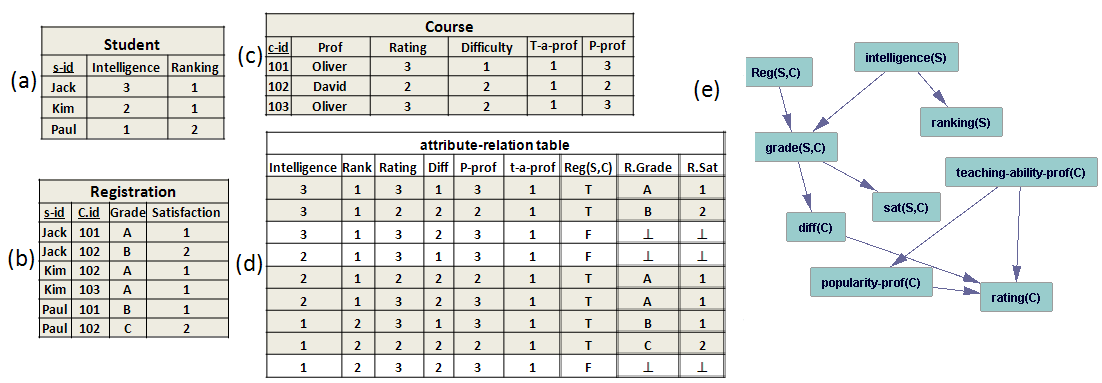
\includegraphics[width=\textwidth]{figures/university-tables3.png} 
  \caption{Database Table Instances: (a) $\student$ (b) $\reg$ (c) $\course$. To simplify, we added the information about professors to the courses that they teach.  (d) The attribute-relation table $\reg^{+}$ derived from $\reg$, which lists for each pair of entities their descriptive attributes, whether they are linked by $\reg$, and the attributes of a link if it exists. (e) A Parametrized Bayes Net for the university schema.}
   \label{fig:university-tables}
\end{figure*}


 The \textbf{natural table join}, or simply join, of two or more tables contains the rows in the Cartesian products of the tables whose values match on common fields. In logical terms, a join corresponds to a conjunction \cite{Ullman1982}. 
 
\section{Bayes Net Learning With Link Correlation Analysis}

We outline the two methods we compare in this paper, flat search and hierarchical search. 

\subsection{Flat Search}
The basic idea for flat search is to apply a standard propositional or single-table Bayes net learner to a single large join table. 
To learn correlations between link types, we need to provide the Bayes net with data about when links are present {\em and} when they are absent. To accomplish this, we add to each relationship table a \textbf{link indicator column}. This columns contains T if the link is present between two entities, and F if the link is absent. (The entities are specified in the primary key fields.) We add rows for all pairs of entities of the right type for the link, and enter T or F in the link indicator column depending on whether a link exists or not. We refer to relationship tables with a link indicator column as \textbf{extended} tables. Extended tables are readily computed using SQL queries. If we omit the entity Ids from an extended table, we obtain the \textbf{attribute-relation} table that lists (1) all attributes for the entities involved, (2) whether a relationship exists and (3) the attributes of the relationship if it exists. If the attribute-relation table is derived from a relationship $R$, we refer to it as $R^{+}$. 

The attribute-relation table is readily defined for a set of relationships: take the cross-product of all populations involved, and add a link indicator column for each relationship in the set.
For instance, if we wanted to examine correlations that involve both the $\reg$ and the $\it{Teaches}$ relationships, we would form the cross-product of the entity types $\it{Student},\it{Course},\it{Professor}$ and build an attribute-relation table that contains two link indicator columns $\reg(\S,\C)$ and $\it{Teaches}(\P,\C)$. 
The \textbf{full join table} is the attribute-relation table for all relationships in the database.
 
The \textbf{flat search Bayes net learner} takes a standard Bayes net learner and applies it to the full join table to obtain a single Parametrized Bayes net.
 The results of \cite{Schulte2011} can be used to provide a theoretical justification for this procedure;
 we outline two key points. \begin{enumerate} \item The full join table correctly represents the {\em sufficient statistics}\cite{Heckerman1995,Schulte2011} of the database: 
using the full join table to compute the frequency of a joint value assignment for Parametrized Random Variables is equivalent to the frequency with which this assignment holds in the database. 
\item Maximizing a standard single-table likelihood score from the full join table is equivalent to maximizing the {\em random selection pseudo likelihood.} 
The random selection pseudo log-likelihood is the expected log-likelihood assigned by a Parametrized Bayes net when we randomly select individuals from each population and instantiate the Bayes net with attribute values and relationships associated with the selected individuals. 
\end{enumerate}

\subsection{Hierarchical Search}
Khosravi {\em et al.} \cite{Schulte2012} present the learn-and-join  structure learning algorithm. 
The algorithm upgrades a single-table Bayes net learner for relational learning. 
We describe the fundamental ideas of the algorithm; for further details please see \cite{Schulte2012}. 
 
The key idea is to build a Bayes net for the entire database by level-wise search through the {\em table join lattice.} The user chooses a single-table Bayes net learner. The learner is applied to table joins of size 1, that is, regular data tables. Then the learner is applied to table joins of size $s,s+1,\ldots$, with the constraint that larger join tables inherit the absence or presence of learned edges from smaller join tables. These edge constraints are implemented by keeping a global cache of forbidden and required edges.  Algorithm~\ref{alg:structure} provides pseudocode for the previous learn-and-join algorithm (LAJ) \cite{Schulte2012c}. 


\begin{figure}[h]
\begin{center}
\resizebox{1\textwidth}{!}{
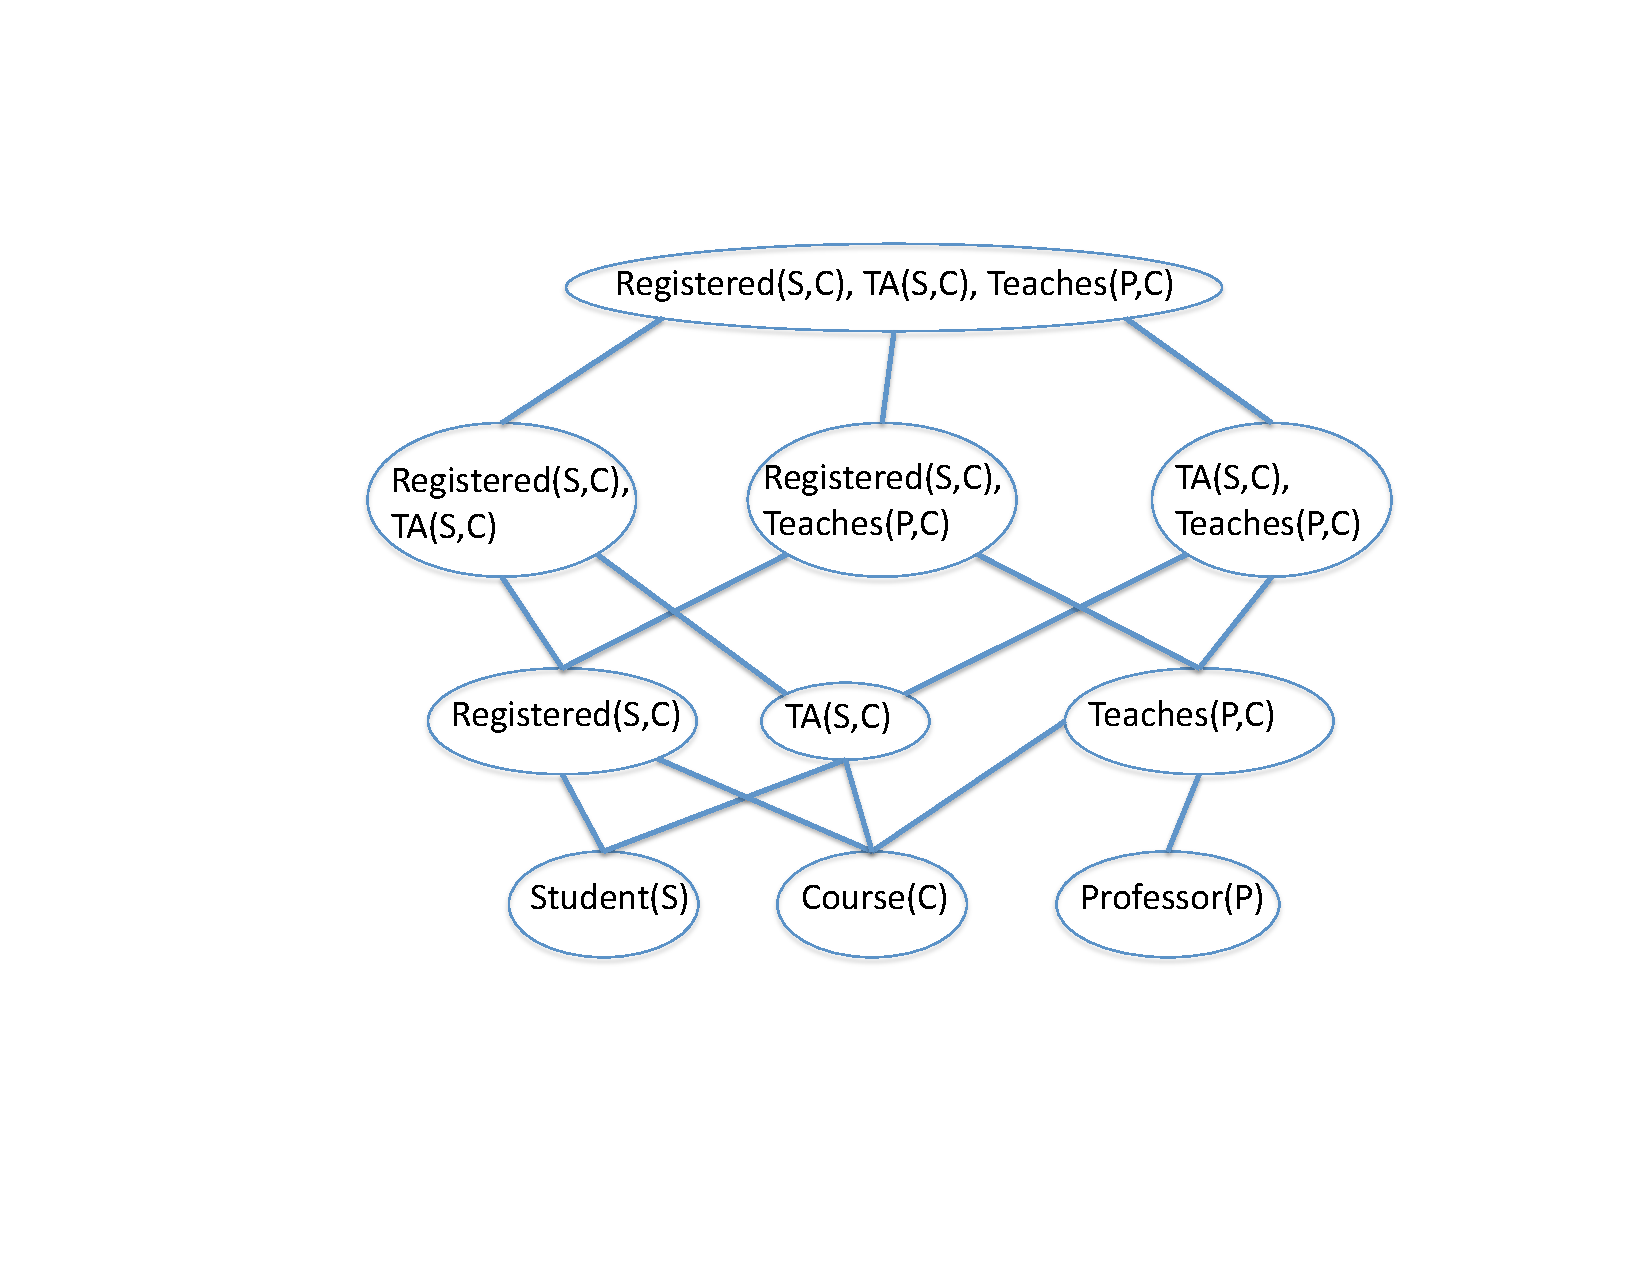
\includegraphics[width=\textwidth]{figures/big-lattice}
}
\caption{A lattice of relationship sets for the university schema of Table~\ref{table:university-schema}.
 Links from entity tables to relationship tables correspond to foreign key pointers. 
%The list representation of the sets is determined by the functor ordering $\it{Registered} < \it{TA} < \it{Teaches}$. 
\label{fig:big-lattice}}
\end{center}
\end{figure}



To extend the learn-and-join algorithm for multiple link analysis, we replace the natural join in line 7 by the extended join (more precisely, by the attribute-relation tables derived from the extended join). 
The natural join contains only tuples that appear in all relationship tables. 
Compared to the extended join, this corresponds to considering only rows where the link indicator columns have the value $\true$. 
When the propositional Bayes net learner is applied to such a table, the link indicator variable appears like a constant. 
Therefore the BN learner cannot find any correlations between the link indicator variable and other nodes, 
nor can it find correlations among attributes conditional on the link indicator variable being $\false$. 
Thus the previous LAJ algorithm finds only correlations between entity attributes conditional on the existence of a relationship. 
In sum, hierarchical search with link correlations can be described as follows.

\begin{enumerate}
\item Run the previous LAJ algorithm (Algorithm~\ref{alg:structure}) using natural joins.
\item Starting with the constraints from step 1, run the LAJ algorithm where extended joins replace natural joins. That is, for each relationship set shown in the lattice of Figure~\ref{fig:big-lattice}, apply the single-table Bayes net learner to the extended join for the relationship set.
\end{enumerate}


\begin{algorithm}[htb]
\begin{algorithmic}
{\footnotesize
\STATE {\em Input}: Database $\D$ with $E_1,..E_e$ entity tables, $R_1,... R_r$ Relationship tables, %ER Model ,
\STATE {\em Output}: Bayes Net for $\D$ 
\STATE {\em Calls}: PBN: Any propositional Bayes net learner that accepts edge constraints and a single table of cases as input. 
\STATE {\em Notation}: PBN$(\T,\mbox{Econstraints})$ denotes the output DAG of PBN. Get-Constraints$(\G)$ specifies a new set of edge constraints, namely that all edges in $\G$ are required, and edges missing between variables in $\G$ are forbidden.
} %fnsize
\end{algorithmic}
\begin{algorithmic}[1]
{\footnotesize
  \STATE Add descriptive attributes of all entity and relationship tables as variables to  $G$. Add a boolean indicator for each relationship table to $G$.
  \STATE Econstraints = $\emptyset$ {[Required and Forbidden edges]} %in the G]}
\FOR {m=1 to e}
  \STATE Econstraints += Get-Constraints(PBN($E_m$ , $\emptyset$)) 
  \ENDFOR 
%\FOR {m=1 to r}
% \STATE Econstraints += Get-Constraints(PBN($R_m$, Econstraints))
%\ENDFOR
\FOR {m=1 to r}
  \STATE $N_m$ :=  natural 
  join of $R_m$ and entity tables linked to $R_m$ 
  \STATE Econstraints += Get-Constraints(PBN($N_m$, Econstraints))
\ENDFOR
\FORALL{$N_i$ and $N_j$ with a foreign key in common}
  \STATE $K_{ij}$ :=  %natural 
  join of $N_i$ and $N_j$ 
  \STATE Econstraints += Get-Constraints(PBN($K_{ij}$, Econstraints))
\ENDFOR
\RETURN Bayes Net defined by Econstraints.

    } %footnotesize
\end{algorithmic}
%\label{alg:cpt}
\caption{Pseudocode for previous Learn-and-Join Structure Learning for Lattice Search. \label{alg:structure}}
\end{algorithm}




\section{Evaluation} 
All experiments were done on a QUAD CPU Q6700 with a 2.66GHz CPU and 8GB of RAM. The LAJ code and datasets are available on the world-wide web \cite{bib:jbnsite}. We made use of the following single-table Bayes Net search implementation:  GES search \cite{Chickering2003} with the BDeu score as implemented in version 4.3.9-0 of CMU's Tetrad package (structure prior uniform, ESS=10; \cite{2008a}).

\paragraph{Methods Compared}

We compared the following methods.

\begin{description}
\item[LAJ] The previous LAJ method without link correlations (Algorithm~\ref{alg:structure}).
\item[LAJ+] The new LAJ method that has the potential to find link correlations (Algorithm~\ref{alg:structure} with the extended join tables instead of natural join tables).
\item[Flat] Applies the single-table Bayes net learner to the full join table.
\end{description}

To implement Flat Search and the LAJ+ algorithm efficiently, we apply the Fast M\"obius Transform to compute tables of sufficient statistics that involve negated relationships. We discuss the details further in Section~\ref{sec:mobius}.

\paragraph{Performance Metrics} We report learning time, log-likelihood, Bayes Information Criterion (BIC), and the Akaike Information Criterion (AIC). BIC and AIC are standard scores for Bayes nets \cite{Chickering2003}, defined as follows. We write 
$$L(\hat{G},\d)$$ for the log-likelihood score,
where $\hat{G}$ is the BN $\G$ with its parameters instantiated to be the maximum likelihood estimates given the dataset $\d$, and the quantity $L(\hat{G},\d)$ is the log-likelihood of $\hat{G}$ on $\d$. 

The BIC score is defined as follows \cite{Chickering2003,Schulte2011}

$$\mathit{BIC}(\G,\d) = L(\hat{G},\d) - \mathit{par}(\G)/2 \times ln(m)$$

where the data table size is denoted by $m$, and $\mathit{par}(\G)$ is the number of free parameters in the structure $\G$. The AIC score is given by 

$$\mathit{AIC}(\G,\d) = L(\hat{G},\d) - \mathit{par}(\G). $$

 Selection by AIC is asympotically equivalent to selection by cross-validation, so we may view it as a closed-form approximation to cross-validation,  which is computationally demanding for relational datasets. 

\begin{table}[btp] \centering
%\scalebox{0.7in}{
%\resizebox{0.5\textwidth}{1.5cm}{
\begin{tabular}[c]
{|p{4cm}|p{3cm}|l|}\hline
    \textbf{Dataset} & \textbf{\#tuples} \\\hline
    University&662\\\hline
    Movielens &1585385\\\hline
    Mutagenesis &1815488\\\hline
    Hepatitis &2965919\\\hline
    %Mondial &59520\\
    %UW-CSE &2099\\
    Small-Hepatitis & 19827 \\\hline
\end{tabular}
%}
 % end scalebox
\setlength{\abovecaptionskip}{10pt}
\caption{Size of datasets in total number of table tuples. 
% \textbf{Zhensong: needs fixing}
 \label{table:datasetsize}}
\end{table}



\paragraph{Datasets}


We used one synthetic and 
three benchmark real-world databases, with the modifications described by Schulte and Khosravi~\cite{Schulte2012}. See that article for more
details.


\noindent\textbf{University Database.} We manually created a small dataset, based on the schema given in Table~\ref{table:university-schema}. 
The dataset is small and is used as a testbed for the correctness of our algorithms.

\noindent\textbf{MovieLens Database.} A dataset from the UC Irvine machine learning repository. The data are organized in 3 tables (2 entity tables, 1 relationship table, and 7 descriptive attributes). 

\noindent\textbf{Mutagenesis Database.} A dataset widely used in ILP research. % \cite{Srinivasan1996}.  
It contains two entity tables and two relationships.

\noindent\textbf{Hepatitis Database.} A modified version of the PKDD'02 Discovery Challenge database. The data are organized in 7 tables (4 entity tables, 3 relationship tables and 16 descriptive attributes). In order to make the learning feasible, we undersampled Hepatitis database to keep the ratio of positive and negative link indicator equal to one. %, following 

\begin{table} \centering
%\scalebox{0.7in}{
%\resizebox{0.5\textwidth}{!}{
\begin{tabular}
{|p{4cm}|c|}\hline 
 \textbf{Dataset} & \textbf{Data Processing Time} \\\hline
University&1.205 \\\hline
Movielens &1.539\\\hline
Mutagenesis &0.723\\\hline
Small-Hepatitis &57.794\\\hline

\end{tabular}
%}
 % end scalebox
\setlength{\abovecaptionskip}{10pt}
\caption{Data Preprocessing: Table Join Time  in seconds. %The Learn-and-Join methods do the same 
%\textbf{Zhensong: needs fixing}
 \label{table:cttimes}}

\end{table}



\begin{table} \centering
%\scalebox{0.7in}{
%\resizebox{0.5\textwidth}{!}{
\begin{tabular}[c]
{|p{4cm}|p{2.1cm}|p{2.1cm}|p{2.1cm}|}\hline
 \textbf{Dataset} & \textbf{Flat} & \textbf{LAJ+} & \textbf{LAJ}\\\hline
University&1.916&1.183&0.291 \\\hline
Movielens &38.767& 18.204& 1.769\\\hline
Mutagenesis &3.231& 3.448& 0.982\\\hline
Small-Hepatitis &9429.884&7.949&10.617 \\\hline
%Mondial &59520&3366 \\ \hline
%UW-CSE &2099&3380 \\ \hline
\end{tabular}
%}
 % end scalebox
\setlength{\abovecaptionskip}{10pt}
\caption{Model Structure Learning Time  in seconds.
% \textbf{Zhensong: needs fixing}
 \label{table:runtimes}}
\end{table}




\subsection{Results} 

\paragraph{Learning Times} Table~\ref{table:cttimes} shows the data preprocessing time that the different methods require for table joins. This is the same for all methods, namely the cost of computing the full join table using the fast M\"obius transform described in Section~\ref{sec:mobius}. 
Table~\ref{table:runtimes}
 provides the model search time for each of the link analysis methods. 
On the smaller and simpler datasets, all search strategies are fast, 
but on the medium-size and more complex datasets (Hepatitis, MovieLens), hierarchical search is much faster due to its use of constraints.


\begin{table}[h]
\begin{center}
\resizebox{1 \textwidth}{!}{
\begin{tabular}{|c|c|c|c|c| }
    \hline \textbf{University} &{BIC}& {AIC} &{log-likelihood} &{\# Parameter}\\
      \hline Flat &-17638.27&-12496.72 & -10702.72& 1767\\
      \hline LAJ+ & -13495.34& -11540.75& -10858.75& 655\\
            \hline LAJ &-13043.17 & -11469.75&-10920.75 & 522\\
      
      \hline
    \end{tabular}
}
\end{center}

\begin{center}
\resizebox{1 \textwidth}{!}{
\begin{tabular}{|c|c|c|c|c| }
    \hline \textbf{MovieLens} &{BIC}& {AIC} &{log-likelihood} &{\# Parameter}\\
      \hline Flat &-4912286.87&-4911176.01 & -4910995.01& 169\\
      \hline LAJ+ & -4911339.74& -4910320.94& -4910154.94& 154\\
            \hline LAJ &-4911339.74 & -4910320.94&-4910154.94 & 154\\
      
      \hline
    \end{tabular}
}
\end{center}


\begin{center}
\resizebox{1 \textwidth}{!}{
\begin{tabular}{|c|c|c|c|c| }
    \hline \textbf{Mutagenesis} &{BIC}& {AIC} &{log-likelihood} &{\# Parameter}\\
      \hline Flat &-21844.67&-17481.03 & -16155.03& 1289\\
      \hline LAJ+ & -47185.43& -28480.33& -22796.33& 5647\\
            \hline LAJ & -30534.26 & -25890.89&-24479.89 & 1374\\
      
      \hline
    \end{tabular}
}
\end{center}

\begin{center}
\resizebox{1 \textwidth}{!}{
\begin{tabular}{|c|c|c|c|c| }
    \hline \textbf{Hepatitis} &{BIC}& {AIC} &{log-likelihood} &{\# Parameter}\\
      \hline Flat &-7334391.72&-1667015.81 & -301600.81& 1365357\\
      \hline LAJ+ & -457594.18& -447740.51& -445366.51& 2316\\
            \hline LAJ &-461802.76& -452306.05&-450018.05    & 2230\\ % updated on April 28th
      
      \hline
    \end{tabular}
}
\end{center}



\caption{Statistical Performance of different Searching Algorithms by dataset.  }
\label{table:result_scores}
\end{table}
\paragraph{Statistical Scores}

As expected, adding edges between link nodes improves the statistical data fit: 
the link analysis methods LAJ+ and Flat perform better than the learn-and-join baseline in terms of log-likelihood on all datasets shown in table~\ref{table:result_scores}, except for MovieLens where the Flat search has a lower likelihood. On the small synthetic dataset University, flat search appears to overfit whereas the hierarchical search methods are very close. On the medium-sized dataset MovieLens, which has a simple structure, all three methods score similarly. Hierarchical search finds no new edges involving the single link indicator node (i.e., LAJ and LAJ+ return the same model). 


\begin{figure*}[htbp] %  figure placement: here, top, bottom, or page
  % \centering
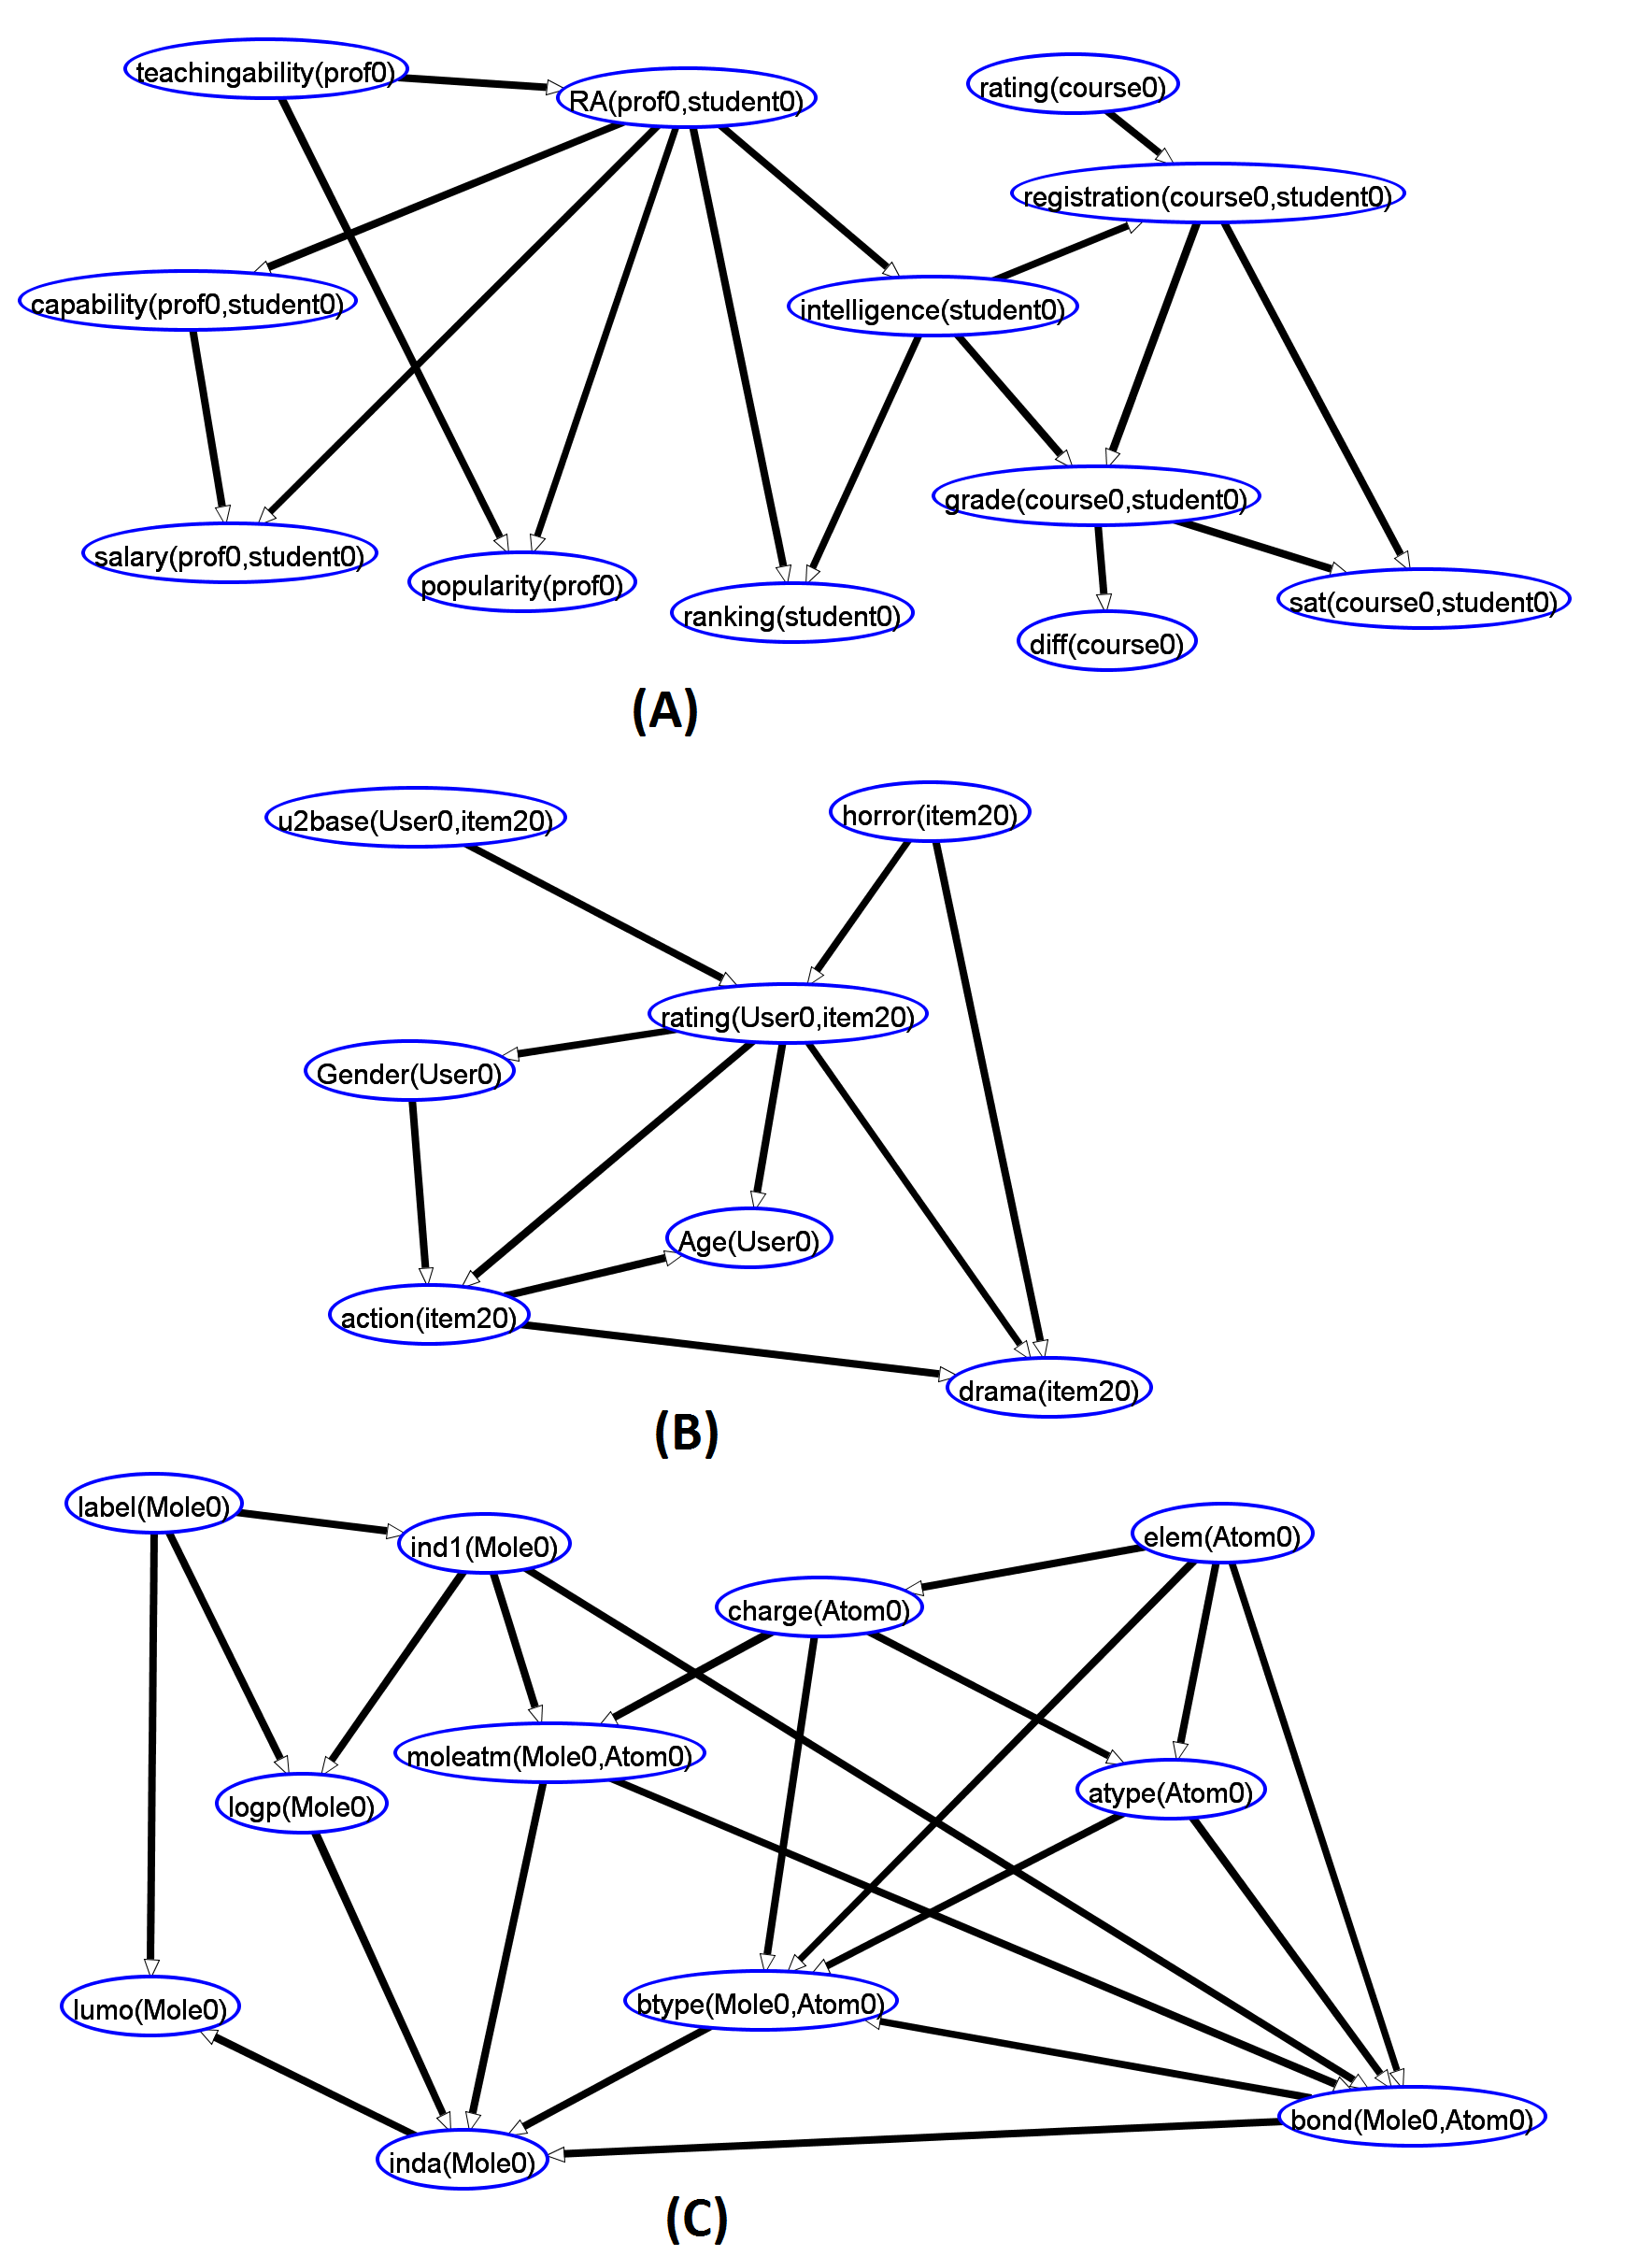
\includegraphics[height=1.0\textheight]{LearnedBN_examples.png}
  \caption{Learned Parametrized Bayes Net for 3 complete datasets: (A) University Database, (B) MovieLens Database, (C) Mutagenesis Database.}
   \label{fig:BN_Examples}
\end{figure*}

The most complex dataset, Hepatitis, is a challenge for flat search, which seems to overfit severely with a huge number of parameters that result in a model selection score that is an order of magnitude worse than for hierarchical search. Because of the complex structure of the Hepatitis schema, the hierarchy constraints appear to be effective in combating overfitting.

The situation is reversed on the Mutagenesis dataset where flat search does well: compared to previous LAJ algorithm, %attribute-only search,
it manages to fit the data better with a less complex model. 
Hiearchical search performs very poorly compared to flat search (lower likelihood yet many more parameters in the model). Investigation of the models shows that the reason for this phenomenon is a special property of the Mutagenesis dataset: The two relationships in the dataset, Bond and MoleAtm, involve the same descriptive attributes. The hierarchical search learns two separate Bayes nets for each relationship, then propagates both sets to the final result. However, the union of the two graphs may not be a compact model of the associations that hold in the entire database. A solution to this problem would be to add a final pruning phase where redundant edges can be eliminated. We expect that with this change, hierarchical search would be competitive with flat search on the Mutagenesis dataset as well.

We also provide learned Bayes net for three databases in terms of the best statistical performance in  Figure~\ref{fig:BN_Examples}.



\section{Computing Data Join Tables} \label{sec:mobius}

The learning algorithms described in this paper rely on the  availability of the extended relational tables $R^{+}$ (see Figure~\ref{fig:university-tables}). A naive implementation constructs this tables using standard joins. However, the cross-products grow exponentially with the number of relations joined, and therefore do not scale to large datasets. In this section we describe a ``virtual join'' algorithm that computes the required data tables without the quadratic cost of materializing a cross-product. 

Our first observation is that Bayes net learners do not require the entire extended table, but  only the {\em sufficient statistics}, namely the counts of how many times each combination of values occurs in the data \cite{Neapolitan2004}. For instance, the attribute-relationship table of Figure~\ref{fig:university-tables}, each combination is observed exactly once. Our second observation is that to compute the sufficient statistics, it suffices to compute the {\em frequencies} of value combinations rather than the counts, because counts can be obtained from frequencies by multiplying with the appropriate domain sizes. An efficient virtual join algorithm for computing frequencies in relational data was recently published by Schulte {\em et al.} \cite{Schulte2013}. Their algorithm is based on the fast M\"obius transform (FMT). We outline it briefly. 


Consider a set of relationship indicator nodes $\R_{1} = \cdot, R_{2} = \cdot,\ldots, R_{m}$ and attribute nodes $\functor_{1},\ldots,\functor_{j}$. The sufficient statistics correspond to a joint distribution over these random variables.

$m$ Boolean relationship random variables:

$$P(\R_{1} = \cdot, R_{2} = \cdot,\ldots, R_{m} = \cdot; \functor_{1} = \cdot,\ldots,\functor_{j} = \cdot).$$

Our goal is to compute sufficient statistics of this form for relational data. The FMT allows us to efficiently find sufficient statistics for binary random variables. We apply it with a fixed set of values for the attribute nodes, which corresponds to a joint distribution over the $m$ Boolean relationship random variables:

$$P(\R_{1} = \cdot, R_{2} = \cdot,\ldots, R_{m} = \cdot; \functor_{1} = v_{1},\ldots,\functor_{j} = v_{j}).$$

The FMT uses the local update operation

\begin{equation}
P(\R = \false, \set{R}) =
P(\set{R}) - P(\R = \true, \set{R})
\label{eq:dynamic}
\end{equation}
where $\set{R}$ is a conjunction of relationship specifications, possibly with both positive and negative relationships. The equation continues to hold if we extend relationship specifications with  any fixed set of value assignments $\functor_{1} = v_{1},\ldots,\functor_{j} = v_{j}$ to attribute functor nodes $\functor_{1},\ldots,\functor_{j}$. Using the convention that $\R = \ast$ means that the value of relationship $\R$ is unspecified, the equation~\eqref{eq:dynamic} can be rewritten as

\begin{equation}
P(\R = \false, \set{R}) =
P(\R=*, \set{R}) - P(\R = \true, \set{R}).
\label{eq:dynamic2}
\end{equation}

\begin{figure}[tb]
\begin{center}
\resizebox{1\textwidth}{!}{
%%!%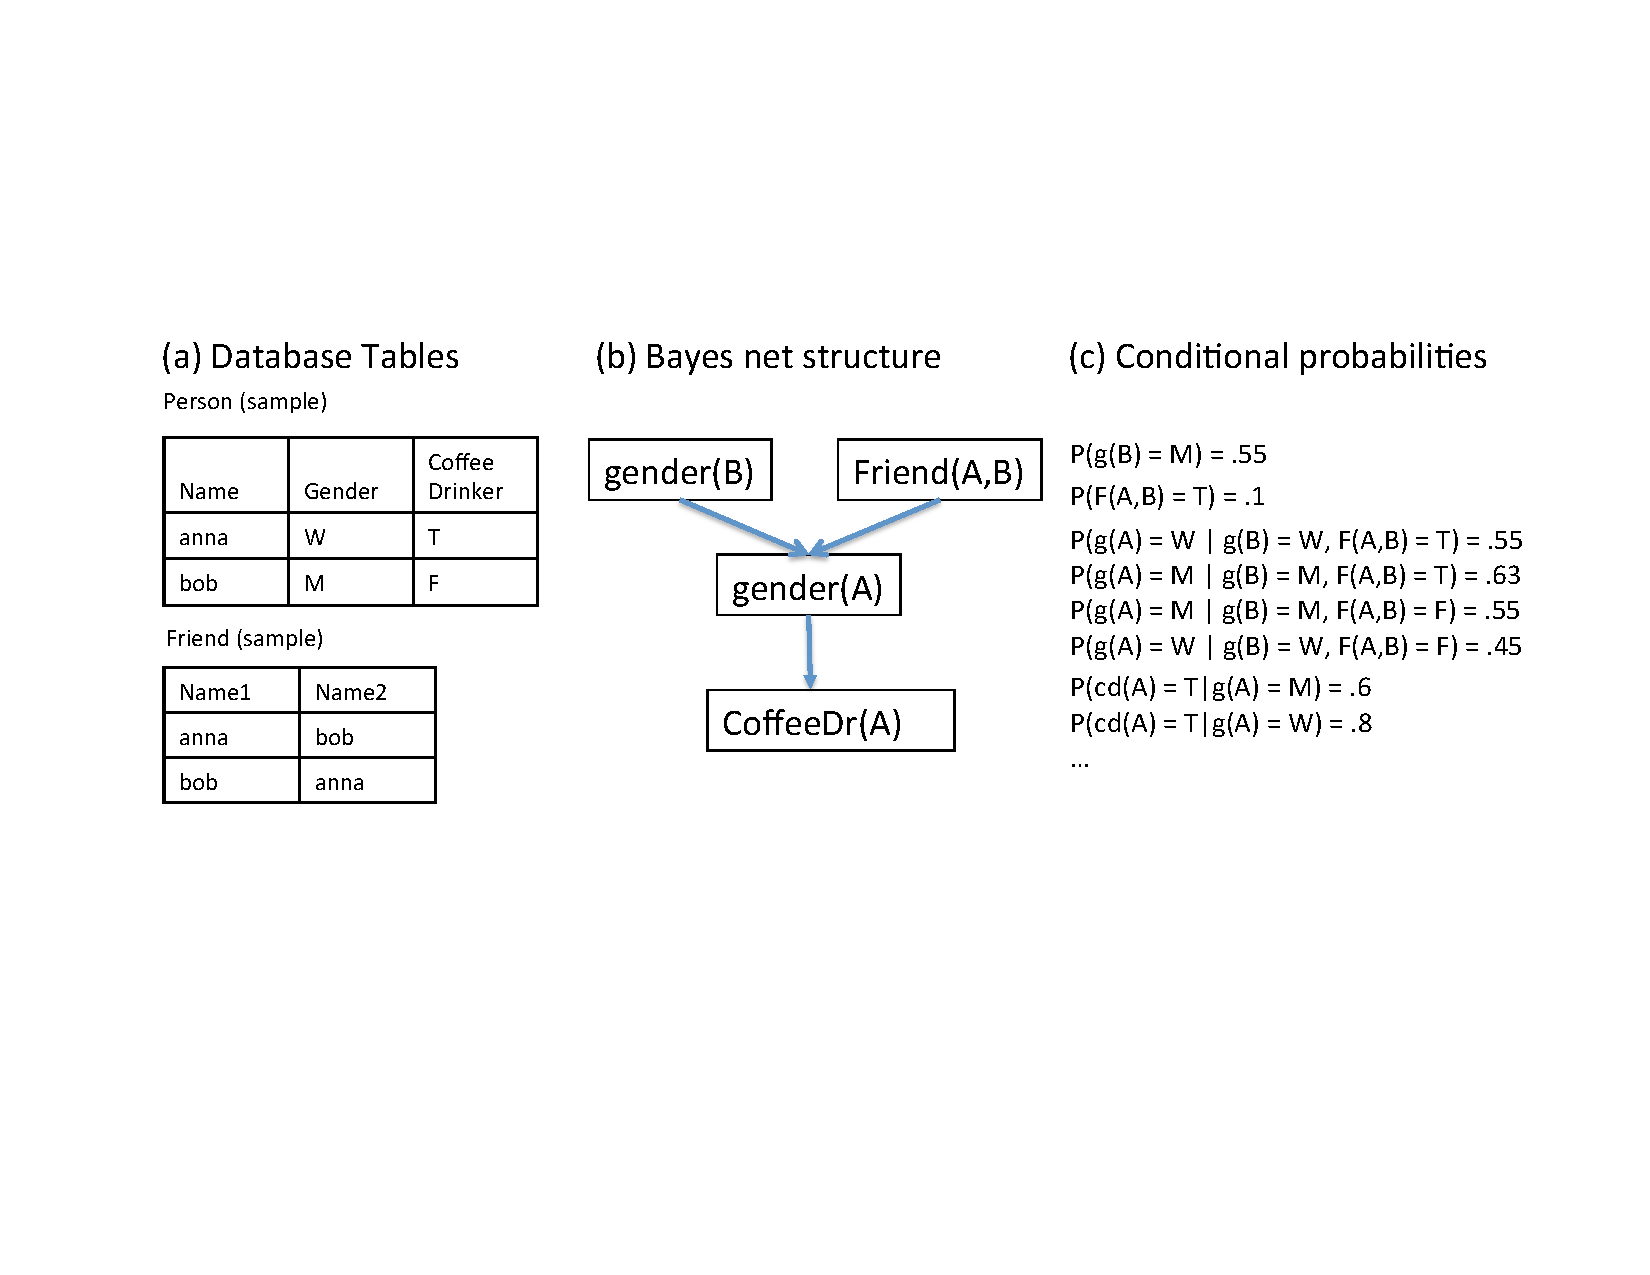
\includegraphics[width=1\textwidth]{pbn}
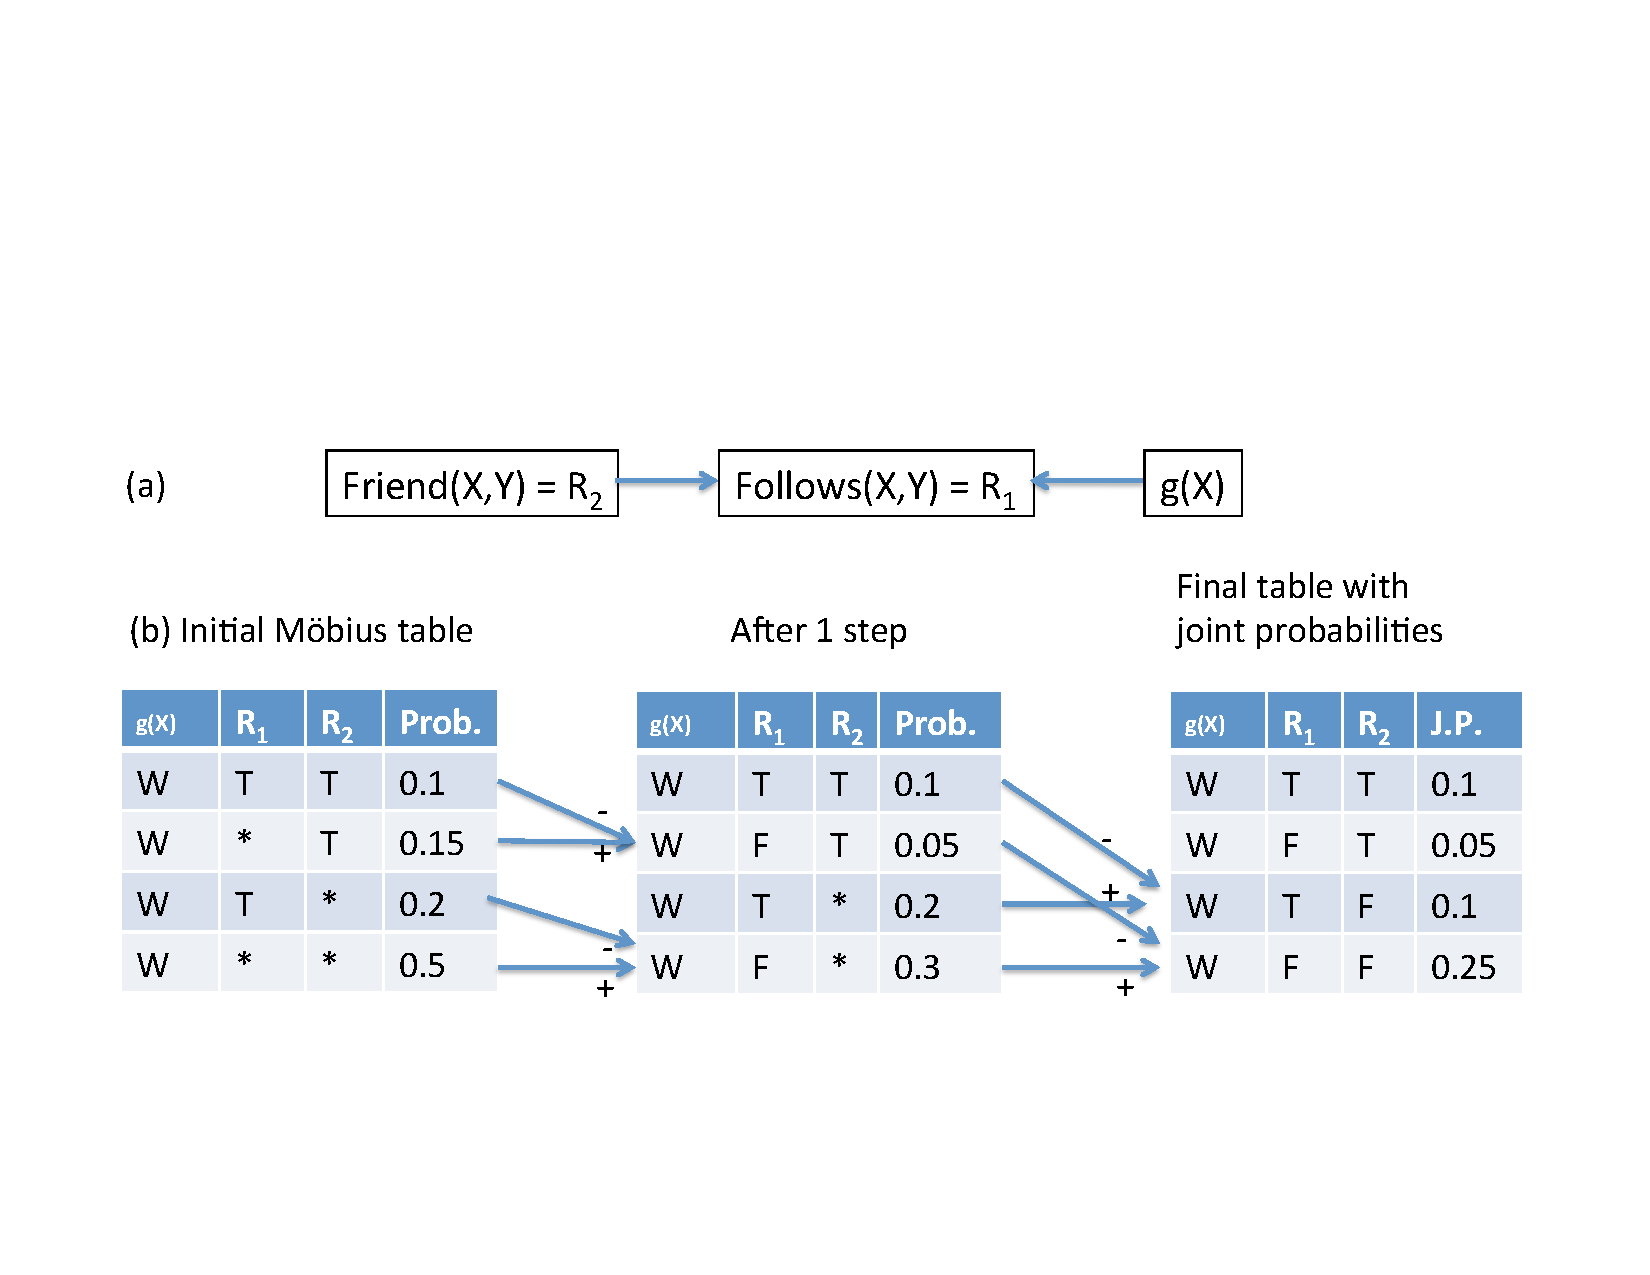
\includegraphics{figures/mobius-v2.pdf}
}
\caption{(a) A Bayes net with two relationship nodes. (b) An illustrative trace of the fast M\"obius transform. 
\label{fig:example}}
\end{center}
\end{figure}

The FMT begins with an initial table of sufficient statistics where all relationship nodes have the value $\true$ or $*$ but not $\false$. Since these sufficient statistics do not involve false relationships, they can be computed efficiently from a relational database using table joins. The procedure then goes through the relationship nodes $\R_{1},\ldots,\R_{m}$ in order, at stage $i$ replacing all occurrences of $\R_{i} = *$ with $\R_{i} = \false$, and applying the local update equation to obtain the probability value for the modified row.
%using Equation~\eqref{eq:dynamic}. 
At termination, all $*$ values have been replaced by $\false$ and the table specifies all joint frequencies as required. Algorithm~\ref{alg:fmt} gives pseudo code and Figure~\ref{fig:example} presents an example of the transform step. For example, the probability entry for the second row of the middle table is computed by applying the equation
\begin{flalign*}
%\begin{eqnarray*}
&P(\R_{1} = \false, \R_{2} = \true; g(\X) = W) = \\
&P(\R_{1} = *, \R_{2} = \true; g(\X) = W) -  P(\R_{1} = \true, \R_{2} = \true; g(\X) = W)  = \\
&0.15 - 0.1 = 0.05
%\end{eqnarray*}
\end{flalign*}  
%\end{footnotesize}
which is an instance of Equation~\eqref{eq:dynamic2}.
\begin{algorithm}[t]
\begin{algorithmic}
%{\footnotesize
%\STATE \underline{Notation}: $\r$ = Assignment for Functor Nodes; \\$\f_{\r}$= the value of 
%$f(t_{1},\ldots,t_{k})$ in row $\r$; \\ $\tau(\r)$ =  probability $\r$ stored in JP-table $\tau$. 
\STATE \underline{Input}: database $\D$; a set of %functor 
nodes divided into attribute nodes $\functor_{1},\ldots,\functor_{j}$ and relationship nodes $\R_{1},\ldots,\R_{m}$.  
%and parent variables divided into a set $\set{\R_{1},\ldots,\R_{m}}$ of relationship predicates and a set $\set{C}$ of function terms that are not relationship predicates.
% \STATE \underline{Calls}: $\join(\set{\C}, \R_1,\cdots,  \R_k)$. Computes join frequencies conditional on relationships $\R_{1},\ldots,\R_{k}$ being true.
\STATE \underline{Output}: joint probability table specifying the data frequencies for each joint assignment to the input 
%functor 
nodes. 
%$\tau$ %such that the entry $\tau(\r)$ for row $\r \equiv
%(\set{\C} = \set{\C}_{\r}, \set{\R} = \set{\R}_{\r})$ is the frequencies $P_{\D}(\set{\C} = \set{\C}_{\r}, \set{\R} = \set{\R}_{\r})$ in the database distribution $\D$.
%}
\end{algorithmic}
\begin{algorithmic}[1]
%{\small
%\STATE \COMMENT{fill in rows with no false relationships using table joins}\label{line:start-join}
\FORALL{attribute value assignments $\functor_{1} := v_{1}, \ldots, \functor_{j} := v_{j}$}
\STATE initialize the table: set all relationship nodes to either $\true$ or $*$; find joint frequencies with data queries.
%\COMMENT{fill in rows with no false relationships using table joins}\label{line:start-join}
\FOR{$i=1$ to $m$}
%\IF[$r$ has $m-i$ unspecified relationships]{$r$ has exactly $i$ true relationships$\R^1,..,\R^i$}
%\STATE find $P_{\D}(\set{\C} =\set{\C}_{\r}, \set{\R} = \set{\R}_{\r})$ using $\join(\set{\C} =\set{\C}_{\r}, \set{\R} = \set{\R}_{\r})$. Store the result in $\tau(\r)$. \label{line:join}
\STATE Change all occurrences of $R_{i} = *$ to $R_{i} = \false$.
\STATE Update the joint frequencies using %Equation
\eqref{eq:dynamic}.
\ENDFOR
\ENDFOR 
%}
\end{algorithmic}
 \caption{The inverse M\"obius transform for parameter estimation in a Parametrized Bayes Net. 
% The algorithm transforms observed frequencies that involve existing (positive) relationships only into a complete set of joint frequencies that involve any combination of positive and negative relationships. 
 %For simplicity we omit nonrelational conditions. 
 \label{alg:fmt}}
\end{algorithm}


\section{Conclusion} We described different methods for extending relational Bayes net learning to correlations involving links. 
Statistical measures indicate that Bayes net methods succeed in finding relevant correlations. 
There is a trade-off between statistical power and computational feasibility (full table search vs constrained search). 
Hierarchical search often does well on both dimensions, but needs to be extended with a pruning step to eliminate redundant edges.

A key issue for scalability is that most of the learning time is taken up by forming table joins, whose size is the cross product of entity tables. 
These table joins provide the sufficient statistics required in model selection. 
To improve scalability, computing sufficient statistics needs to be feasible for cross product sizes in the millions or more. 
A  solution is applying virtual join methods that compute sufficient statistics without materializing table joins, such as the Fast M\"obius Transform~\cite{Schulte2012b,Yin2004}.

A valuable direction for future work is to compare learning link correlations with directed and undirected models, such as Markov Logic Networks \cite{Domingos2009}. As we explained in Section~\ref{sec:related}, current relational learners for undirected models do not scale to most of our datasets. One option is to subsample the datasets so that we can compare the statistical power of directed and undirect learning methods
independently of scalability issues. Khosravi {\em et al.} were able to obtain structure learning results for Alchemy~\cite{Khosravi2010}, but did not evaluate the models with respect to link correlations. For the MLN-Boost system, we were able to obtain preliminary results on several benchmark databases  (including Mutagenesis and Hepatitis), by selecting the right subset of target predicates. MLN-Boost is the current state-of-the-art learner for Markov Logic Networks \cite{Khot2011}. The Bayes net models were competitive with the MLN-Boost models on a standard cross-validation measure of predictive accuracy.

\bibliography{master_lncs_gkr}
\bibliographystyle{plain}
\end{document}
